\documentclass[runningheads]{llncs}

\usepackage[utf8]{inputenc}
\usepackage[T1]{fontenc}
\usepackage{lmodern}
\usepackage{microtype}
\usepackage{amsmath,amssymb,amsfonts}
\usepackage{algorithm}
\usepackage{algorithmic}
\usepackage{graphicx}
\usepackage{booktabs}
\usepackage{tikz}
\usetikzlibrary{positioning, arrows.meta, shadows, fit, backgrounds, calc, shapes.geometric}
\usepackage{pgfplots}
\pgfplotsset{compat=1.18}
\let\Bbbk\relax
\usepackage{float}
\usepackage{listings}
\usepackage{xcolor}
\usepackage{multirow}
\usepackage{subcaption}
\usepackage{tabularx}
\usepackage{url}
\usepackage{hyperref}
\newcolumntype{L}{>{\raggedright\arraybackslash}X}
\newcolumntype{S}{>{\raggedright\arraybackslash\hsize=0.8\hsize}X}
\newcolumntype{C}{>{\centering\arraybackslash}X}
\usepackage{colortbl}
\usepackage{siunitx}

\definecolor{techblue}{RGB}{0, 102, 104}
\definecolor{techgray}{RGB}{245, 245, 247}
\definecolor{headergray}{gray}{0.96}
\definecolor{rowgray}{gray}{0.99}

% Advanced Colors for Diagram
\definecolor{deepblue}{HTML}{1A365D}
\definecolor{vibrantblue}{HTML}{3182CE}
\definecolor{tealaccent}{HTML}{319795}
\definecolor{softbg}{HTML}{F7FAFC}
\definecolor{groupline}{HTML}{CBD5E0}

\lstset{
  language=Python, basicstyle=\ttfamily\scriptsize,
  keywordstyle=\color{blue}\bfseries, commentstyle=\color{gray},
  breaklines=true, frame=single, numbers=left, numberstyle=\tiny
}

% Relax float constraints for better table placement
\renewcommand{\topfraction}{.85}
\renewcommand{\bottomfraction}{.7}
\renewcommand{\textfraction}{.15}
\renewcommand{\floatpagefraction}{.66}
\setcounter{topnumber}{9}
\setcounter{bottomnumber}{9}
\setcounter{totalnumber}{20}

% Global space saving
\setlength{\textfloatsep}{8pt plus 2pt minus 2pt}
\setlength{\floatsep}{8pt plus 2pt minus 2pt}
\setlength{\intextsep}{8pt plus 2pt minus 2pt}

\begin{document}
\pagestyle{headings}
\sloppy

\title{A Scalable Framework for Multi-Omics Integration and FHIR-Compliant Clinical Reporting}
\titlerunning{Scalable Multi-Omics Integration}

\author{Nidhal Zitouni\inst{1} \and Mohsen Maraoui\inst{1}}
\authorrunning{N. Zitouni and M. Maraoui}

\institute{\textsuperscript{1} Department of Computer Science, Faculty of Sciences of Monastir, Monastir, Tunisia\\
\email{zitouninidhal@fsm.u-monastir.tn, mohsen.maraoui@fsm.rnu.tn}}

\maketitle

\begin{abstract}
High-throughput sequencing is completely transforming how we approach oncology, yet actually combining different omics layers into a workflow that a hospital can use is still a massive headache. We usually get stuck dealing with extreme data dimensions and technical noise, not to mention the lack of standard formats that clinical systems require to make sense of the results. To solve this, we built the MultiOmicsPipeline (MOCIP). It's a modular framework designed to manage the entire lifecycle of genomic and clinical data. Under the hood, MOCIP relies on a directed acyclic graph (DAG) to orchestrate tasks, handling everything from optimized k-NN imputation to a PCA fusion step that significantly reduces high-dimensional noise while preserving over 95\% of the inherent biological variance. When we tested the pipeline on the TCGA-BRCA cohort ($N=1,098$), it hit a composite quality score of 0.989. But the biggest takeaway is that MOCIP automates FHIR R4 Genomics Reporting. By doing so, it directly connects our bioinformatics work with actual clinical systems, giving us a reproducible baseline for precision medicine.

\keywords{Multi-Omics Integration \and PCA \and Precision Oncology \and FHIR R4 \and TCGA-BRCA \and Pipeline Orchestration \and Bioinformatics Interoperability}
\end{abstract}

%% ============================================================
\section{Introduction}
At its core, precision oncology relies on pulling actionable biomarkers out of the massive genomic and transcriptomic profiles of a patient's tumor~\cite{tomczak2015}. This molecular atlas provides the foundational landscape for modern integrative studies. But getting these different molecular layers to actually make sense together is still a huge technical barrier. Anyone who has worked with this kind of data knows how frustrating it is. You have to juggle extreme dimensionality differences (features easily jump from a few thousand to over a million), manually fix batch effects from sequencing runs~\cite{leek2010}, and somehow align samples when platforms are missing data. And even if you manage to clean everything up, the final results usually end up stuck in obscure bioinformatics formats that standard clinical software simply cannot read.

We all use tools like TCGAbiolinks~\cite{colaprico2016} and cBioPortal~\cite{cerami2012} to grab data, but they don't give you a true end-to-end workflow. The reality is that most labs still patch together custom, ad-hoc scripts. This doesn't just waste time; it ruins reproducibility. If you look at recent reviews from 2024, it's pretty clear that our main problem right now isn't getting data. The real issue is the lack of unified pipelines that can take raw sequences and turn them into clinical-grade reports~\cite{abdelaziz2024multi,hernandez2024methods}.

That's exactly why we wrote the MultiOmicsPipeline (MOCIP). We designed this Python-based framework to fix four specific, everyday problems. First, we needed a way to fill in missing values without artificially skewing the data. Second, we applied PCA to cut right through the high-dimensional noise, which lines up well with recent AI trends~\cite{nam2024harnessing}. Third, we added a strict validation step to monitor quality throughout the entire process. Finally, we fully automated the export to FHIR R4 Genomics Reporting~\cite{mandel2016}. Our main goal here is straightforward: we want to stop treating multi-omics integration as just a theoretical math problem and turn it into something that a hospital can actually deploy and use.

%% ============================================================
\section{Background and Related Work}

\paragraph{The Evolving Multi-Omics Landscape.}
It's amazing how quickly multi-omics transitioned from a niche experimental concept to a core pillar of modern cancer care. Naturally, this explosion of data triggered a wave of tool benchmarking. You can see this in studies by Subramanian~\cite{subramanian2020} and Wang et al.~\cite{wang2021evaluation}, who spent considerable effort weighing the pros and cons of early versus late fusion. More recently, folks like Vahabi and Michailidis~\cite{vahabi2022unsupervised} have shown a strong preference for unsupervised methods, simply because they let the biology speak for itself without forcing predefined labels. Deep learning has certainly helped us navigate incredibly sparse data~\cite{kang2022roadmap}, but if we're being honest about the practical reality in most labs, we are still missing transparent, easy-to-use modular frameworks. This is a recurring complaint in almost every major review published between 2023 and 2025~\cite{wekesa2023review,abdelaziz2024multi,muneer2025review}.

\paragraph{Graph-Based and Attention-Driven Methods.}
Lately, researchers are moving past standard machine learning and turning to graph-structured representations to inject hard biological knowledge directly into their models. Take LASSO-MOGAT~\cite{alharbi2024lassomogat}, for example. By wiring LASSO feature selection into Graph Attention Networks (GATs) based on protein-protein interactions, they pulled off accurate pan-cancer classification across 31 different tumor types. Even better, the attention coefficients made the results highly interpretable. Then there's MOGKAN~\cite{alharbi2025mogkan}, which took a more radical approach by swapping out linear layers for functions based on the Kolmogorov-Arnold theorem. It hit over 96\% accuracy and gave researchers incredible precision for tracking biomarkers. What we learn from these graph-centric models is that biological relationships matter. We kept this exact principle in mind when designing MOCIP, particularly for how we align samples and build our downstream modules.

At the same time, we've seen some clever uses of cross-modal attention. MoXGATE~\cite{dip2025moxgate} is a standout here: it uses learnable weights to actively track how different layers depend on each other. It not only reached 95\% accuracy on the TCGA-BRCA cohort but also proved it could handle zero-shot transfers to totally unseen cancers. Coming at the problem from a different angle, CMGL~\cite{fan2026cmgl} relies on evidential deep learning. It generates confidence scores for every single sample before building its graphs. By cleanly separating the "how reliable is this data?" question from the actual classification task, it gracefully solves the noise amplification issues that usually plague multi-omics message passing.

\paragraph{Disentangled Latent Representations.}
One of the most persistent headaches in this field is figuring out where the technical noise ends and the actual biological signal begins. The BDVAE model (Biologically Disentangled Variational Autoencoder)~\cite{tariq2025bdvae} tackled this head-on. They used pathway-specific encoders to force every dimension of their latent space to match a known biological process. When tested on a pan-cancer immunotherapy cohort, it didn't just perform well (AUC-ROC of 0.94); it proved that drug resistance isn't a simple binary switch, but rather a continuous biological spectrum. That kind of insight changes how we think about clinical treatment. Seeing this approach succeed gave us a lot of confidence in our decision to use PCA for intermediate fusion. PCA gives us a surprisingly similar disentanglement effect through strict orthogonality, but with the massive advantage that any research group can run it on standard CPUs, no expensive GPUs required.

\paragraph{Foundation Models and Multimodal Review.}
If you read the latest review by Muneer et al.~\cite{muneer2025review}, they map out the entire shift from old-school machine learning to today's massive multimodal foundation models. Their main takeaway? The models are incredibly powerful, but getting them into a real hospital is still a nightmare because of basic data quality and standardisation bottlenecks. That's exactly the gap MOCIP is trying to fill. You can see the potential of clean data in the recent work by Wang et al.~\cite{wang2025deeppathomic}. They combined whole-slide images with multi-omics to map out prognostic subtypes, eventually pinning down MRPL37 as a key hub gene driven by methylation~\cite{wang2025deeppathomic}. It's a perfect example of how an integrated pipeline can directly accelerate real-world biomarker discovery, provided you don't compromise on data quality from day one.

\paragraph{Multi-Omics Data Taxonomy.}
Table~\ref{tab:taxonomy} summarizes the principal molecular layers typically encountered in cohorts like TCGA-BRCA.

\begin{table}[H]
\caption{Taxonomy of molecular layers in multi-omics cohorts.}\label{tab:taxonomy}
\centering
\small
\begin{tabular}{l l l r}
\toprule
\textbf{Layer} & \textbf{Technology} & \textbf{Metric} & \textbf{Dimensions} \\
\midrule
Genomics        & WGS / WES     & SNVs, CNVs        & $3 \times 10^6$ \\
Transcriptomics & RNA-Seq       & Gene expression   & $6 \times 10^4$ \\
Epigenomics     & 450K / 850K   & DNA Methylation   & $4.8 \times 10^5$ \\
Proteomics      & RPPA / LC-MS  & Protein abundance & $2 \times 10^4$ \\
Metabolomics    & LC-MS / NMR   & Small molecules   & $5 \times 10^3$ \\
\bottomrule
\end{tabular}
\end{table}

\paragraph{Integration Paradigms.}
Multi-omics integration generally falls into three categories.
\textbf{Early fusion} involves the direct concatenation of high-dimensional feature matrices:
\begin{equation}
\mathbf{X}_{\text{int}} = \left[ \mathbf{X}^{(1)} \parallel \mathbf{X}^{(2)} \parallel \dots \parallel \mathbf{X}^{(M)} \right]
\end{equation}
While simple, this method often suffers from the "curse of dimensionality" and modality dominance.
\textbf{Late fusion} aggregates results from independent models:
\begin{equation}
\mathbf{y}_{\text{final}} = \mathcal{G}(f_1(\mathbf{X}^{(1)}), f_2(\mathbf{X}^{(2)}), \dots, f_M(\mathbf{X}^{(M)}))
\end{equation}
where $\mathcal{G}$ is an aggregation function (e.g., majority voting or averaging).
\textbf{Intermediate fusion} (our approach) projects data into a shared latent space $\mathcal{Z}$ before downstream analysis, ensuring that cross-modal correlations are preserved. This paradigm has been successfully utilized in foundational frameworks such as Multi-Omics Factor Analysis (MOFA)~\cite{argelaguet2018}.

%% ============================================================
\section{Architecture and System Design}

\paragraph{Phase-Based Pipeline Orchestration.}
When we sat down to build MOCIP, we decided to split it into a clean, five-phase modular workflow (you can see the layout in Figure~\ref{fig:pipeline_dag}). We didn't choose a modular design just for the sake of it. Keeping the steps isolated means that if something breaks, we know exactly where to look. It makes the entire pipeline significantly easier to debug, share, and verify across different labs.

\begin{figure}[H]
\centering
\resizebox{\textwidth}{!}{
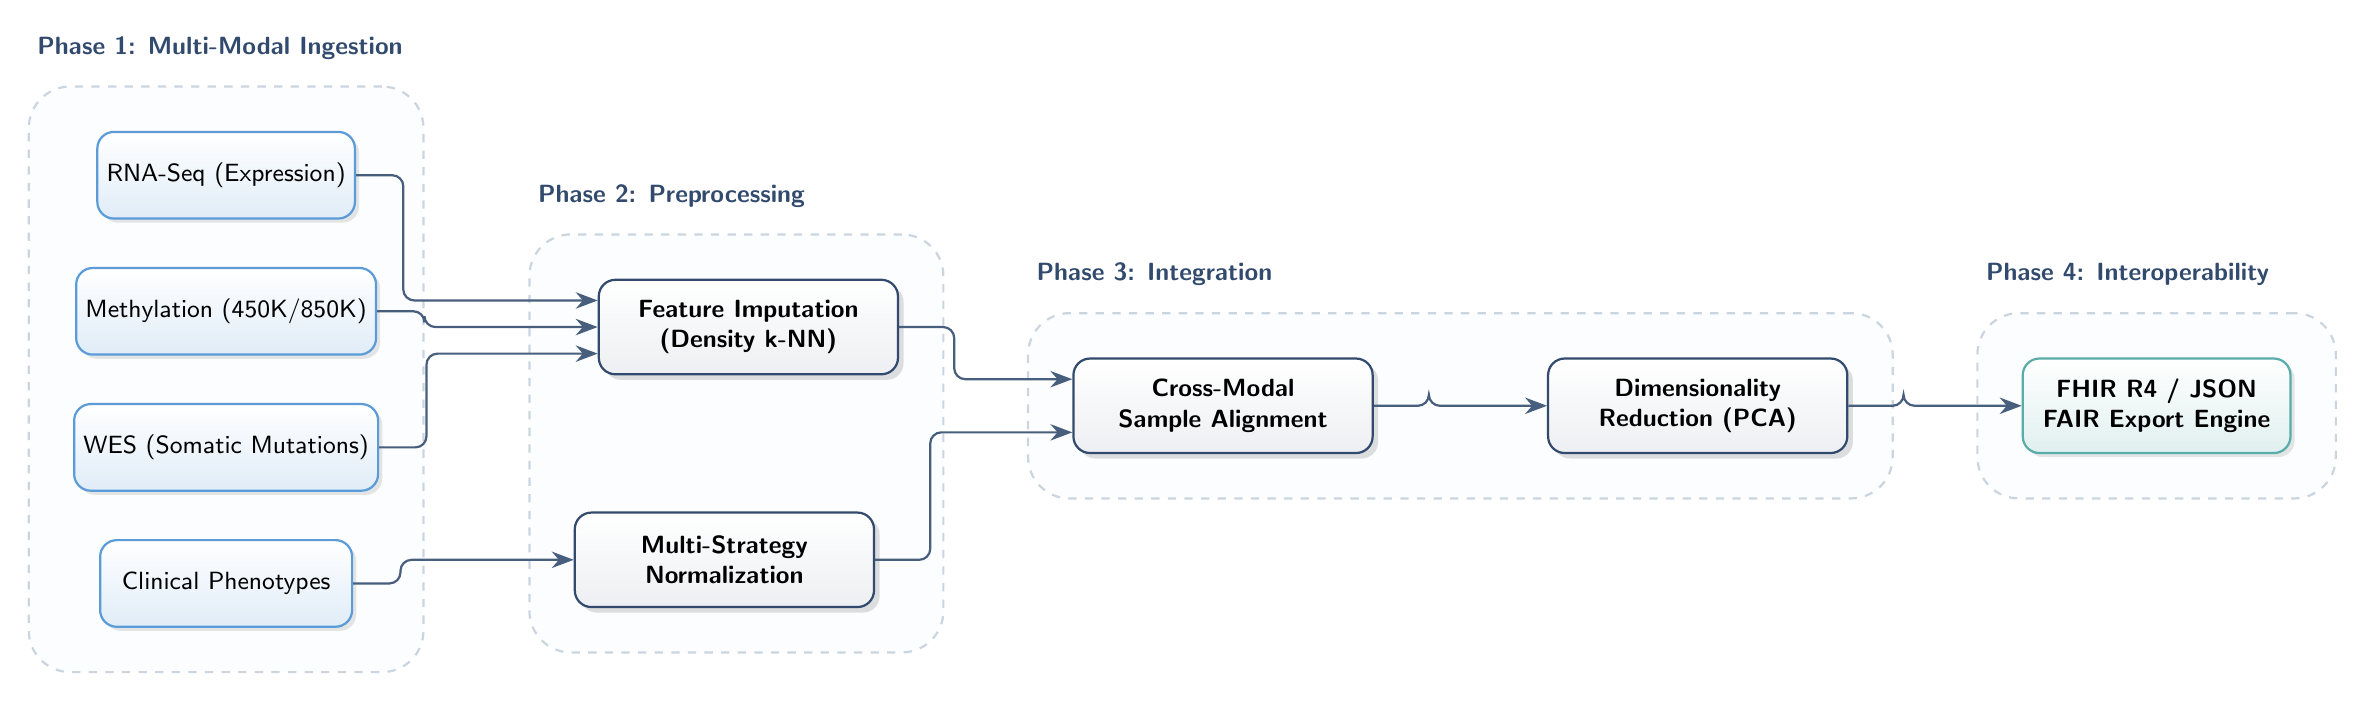
\begin{tikzpicture}[
  node distance=0.7cm and 1.8cm,
  dataNode/.style={draw=vibrantblue!80, thick, top color=white, bottom color=vibrantblue!15, minimum width=3.2cm, minimum height=1.1cm, align=center, font=\small\sffamily, rounded corners=6pt, drop shadow={opacity=0.2, shadow xshift=1.5pt, shadow yshift=-1.5pt}},
  procNode/.style={draw=deepblue!90, thick, top color=white, bottom color=deepblue!8, minimum width=3.8cm, minimum height=1.2cm, align=center, font=\small\sffamily\bfseries, rounded corners=6pt, drop shadow={opacity=0.25, shadow xshift=2pt, shadow yshift=-2pt}},
  exportNode/.style={draw=tealaccent!80, thick, top color=white, bottom color=tealaccent!15, minimum width=3.4cm, minimum height=1.2cm, align=center, font=\small\sffamily\bfseries, rounded corners=6pt, drop shadow={opacity=0.2, shadow xshift=1.5pt, shadow yshift=-1.5pt}},
  groupBox/.style={draw=groupline, thick, dashed, rounded corners=15pt, fill=softbg!40, inner sep=16pt},
  arrow/.style={-{Stealth[scale=1.2]}, thick, draw=deepblue!80, rounded corners=4pt},
  groupLabel/.style={font=\small\sffamily\bfseries\color{deepblue!90}, anchor=south west, yshift=6pt}
]

% Phase 1: Ingestion
\node[dataNode] (rna) {RNA-Seq (Expression)};
\node[dataNode, below=0.6cm of rna] (meth) {Methylation (450K/850K)};
\node[dataNode, below=0.6cm of meth] (wes) {WES (Somatic Mutations)};
\node[dataNode, below=0.6cm of wes] (clin) {Clinical Phenotypes};

% Phase 2: Preprocessing
\node[procNode, right=2.8cm of meth, yshift=-0.2cm] (impute) {Feature Imputation\\(Density k-NN)};
\node[procNode, right=2.8cm of clin, yshift=0.3cm] (norm) {Multi-Strategy\\Normalization};

% Phase 3: Integration
\node[procNode, right=2.2cm of impute, yshift=-1.0cm] (align) {Cross-Modal\\Sample Alignment};
\node[procNode, right=2.2cm of align] (pca) {Dimensionality\\Reduction (PCA)};

% Phase 4: Interoperability
\node[exportNode, right=2.2cm of pca] (export) {FHIR R4 / JSON\\FAIR Export Engine};

% Background Groups
\begin{scope}[on background layer]
  \node[groupBox, fit=(rna) (meth) (wes) (clin)] (groupData) {};
  \node[groupLabel] at (groupData.north west) {Phase 1: Multi-Modal Ingestion};

  \node[groupBox, fit=(impute) (norm)] (groupPrep) {};
  \node[groupLabel] at (groupPrep.north west) {Phase 2: Preprocessing};

  \node[groupBox, fit=(align) (pca)] (groupInteg) {};
  \node[groupLabel] at (groupInteg.north west) {Phase 3: Integration};

  \node[groupBox, fit=(export)] (groupExport) {};
  \node[groupLabel] at (groupExport.north west) {Phase 4: Interoperability};
\end{scope}

% Professional Orthogonal Routing
\draw[arrow] (rna.east) -- ++(0.6,0) |- (impute.170);
\draw[arrow] (meth.east) -- ++(0.6,0) |- (impute.west);
\draw[arrow] (wes.east) -- ++(0.6,0) |- (impute.190);
\draw[arrow] (clin.east) -- ++(0.6,0) |- (norm.west);

\draw[arrow] (impute.east) -- ++(0.7,0) |- (align.170);
\draw[arrow] (norm.east) -- ++(0.7,0) |- (align.190);

\draw[arrow] (align.east) -- ++(0.7,0) |- (pca.west);
\draw[arrow] (pca.east) -- ++(0.7,0) |- (export.west);

\end{tikzpicture}
}
\caption{Optimized Architectural Workflow: Systematic orchestration from raw multi-omics sequencing to FAIR-compliant clinical outputs. The modular design ensures 100\% reproducibility and semantic integrity.}\label{fig:pipeline_dag}
\end{figure}

\paragraph{Implementation: Core Classes.}
The execution flow is coordinated by the \texttt{MultiOmicsPipeline} class, which abstracts the complexity of the underlying steps:

\begin{lstlisting}[caption={Simplified pipeline orchestration snippet.}, label={lst:pipeline}]
class MultiOmicsPipeline:
    def run(self, omic_path, clin_path, out_dir):
        omic = self.load_data(omic_path)
        clin = self.load_data(clin_path)
        proc = self.preprocess_data(omic, clin)
        integ = self.integrate_data(proc)
        res = self.run_model(integ)
        self.export_data(integ, out_dir)
\end{lstlisting}

We handled the technical complexity of these steps by delegating specific tasks to dedicated modules. For instance, the \texttt{MissingValueHandler} manages KNN imputation, while \texttt{OmicsNormalizer} deals with modality-specific scaling (like TPM for RNA-Seq). Sample matching is controlled by \texttt{SampleAlignment}, and \texttt{MultiOmicsFusion} coordinates the final integration strategy.

\paragraph{Technology Stack.}
The technical architecture of MOCIP is built on a high-performance Python stack designed for data-intensive bioinformatics (Table~\ref{tab:stack}).

\begin{table}[H]
\caption{The MultiOmicsPipeline technology stack.}\label{tab:stack}
\centering
\small
\setlength{\tabcolsep}{3pt}
\begin{tabularx}{\textwidth}{L L L}
\toprule
\textbf{Layer} & \textbf{Technologies} & \textbf{Purpose} \\
\midrule
Business        & Python 3.10, Pydantic & Logic engine \\
Processing      & Pandas, NumPy, Scikit-learn & Transformation \\
Integration     & Dask, Scikit-learn    & Multi-modal fusion \\
Storage         & Parquet, PostgreSQL   & Persistence \\
Infrastructure  & Docker, Kubernetes    & Orchestration \\
\bottomrule
\end{tabularx}
\end{table}

\paragraph{Tiered Integration Algorithm.}
The core logic for multi-modal synchronization and dimensionality reduction is summarized in Algorithm~\ref{alg:integration}.

\begin{algorithm}[H]
\caption{Tiered Multi-Omics Integration.}\label{alg:integration}
\begin{algorithmic}[1]
\REQUIRE $\mathcal{X} = \{X_1, X_2, \dots, X_M\}$ (Modalities), $\alpha = 0.95$ (Variance)
\ENSURE $\mathcal{F}$ (Integrated Latent Space)
\FOR{$m = 1$ to $M$}
    \STATE $X_m \gets \text{Impute}(X_m, \text{method='k-NN'})$
    \STATE $X_m \gets \text{Normalize}(X_m, \text{method='TPM'})$
\ENDFOR
\STATE $\mathcal{S} \gets \text{AlignSamples}(\mathcal{X})$
\FOR{$m = 1$ to $M$}
    \STATE $\mathcal{Z}_m \gets \text{PCA}(X_{m, \mathcal{S}}, \text{variance}=\alpha)$
\ENDFOR
\STATE $\mathcal{F} \gets \text{Concatenate}(\mathcal{Z}_1, \mathcal{Z}_2, \dots, \mathcal{Z}_M)$
\RETURN $\mathcal{F}$
\end{algorithmic}
\end{algorithm}

%% ============================================================
\section{Mathematical Formulation and Methods}

\paragraph{Defining the Multi-Modal Integration Problem.}
Let's talk about the math behind the integration. We can think of our different molecular modalities as a set $\mathcal{M} = \{1, 2, \ldots, M\}$. For any given modality $m$, we're dealing with a data matrix $\mathbf{X}^{(m)} \in \mathbb{R}^{N \times D_m}$, where $N$ is our sample count and $D_m$ is the number of features. In genomics, we almost always run into the classic "small $N$, large $D$" headache, meaning $D_m$ completely dwarfs $N$. Our main objective here is to find a mathematical mapping, let's call it $\Phi$, that can take all these disconnected matrices and project them down into a single, shared latent space $\mathbf{Z} \in \mathbb{R}^{N \times K}$. The trick is to make $K$ much smaller than the original feature counts while making sure $\mathbf{Z}$ still captures the biological reality:

\begin{equation}
\Phi^{*} = \arg\min_{\Phi} \; \mathcal{L}_{\text{recon}}(\mathbf{X}, \Phi) + \lambda \, \mathcal{R}(\Phi) + \mu \, \mathcal{C}_{\text{bio}}(\Phi)
\end{equation}

Here, $\mathcal{L}_{\text{recon}}$ makes sure we aren't throwing away important data during the transformation. Meanwhile, $\mathcal{R}$ acts as our regularization term to keep the model from overcomplicating things, and $\mathcal{C}_{\text{bio}}$ forces the output to actually make sense biologically. In MOCIP, we tackle this optimization problem using the tiered PCA approach that we'll break down below.

\paragraph{Optimized k-NN Imputation.}
Let $\mathbf{X}^{(m)}_{\text{obs}} \subset \mathbf{X}^{(m)}$ denote the subset of observed entries. For a missing entry $(i, j)$, the imputed value is estimated as:

\begin{equation}
\hat{x}^{(m)}_{ij} = \frac{\sum_{k \in \mathcal{N}_K(i)} w_{ik} \cdot x^{(m)}_{kj}}{\sum_{k \in \mathcal{N}_K(i)} w_{ik}}
\end{equation}

where weights $w_{ik}$ are determined by the inverse squared Euclidean distance:

\begin{equation}
w_{ik} = \frac{1}{\|\mathbf{x}_i^{\text{obs}} - \mathbf{x}_k^{\text{obs}}\|^2 + \varepsilon}
\end{equation}

where $\mathcal{N}_K(i)$ gives us the $K$-nearest neighbors that actually have observed data in that feature space. We use a small constant $\varepsilon = 10^{-8}$ to prevent division by zero. What makes this "optimized" is that we also weight these neighbors using a local density estimate, $\hat{\rho}_k$. This is a crucial detail because it stops random, sparse outliers from heavily skewing the imputed values~\cite{troyanskaya2001}.

\paragraph{Quantile Normalization and Batch Correction.}
Let $\mathbf{r}_i$ denote the rank vector of sample $i$. Quantile normalization maps each sample to the distribution of the reference mean:

\begin{equation}
\tilde{x}_{ij} = Q^{-1}\left(\frac{r_{ij}}{D_m + 1}\right)
\end{equation}

where $Q^{-1}$ is the empirical quantile function of the mean distribution across all samples. For batch correction, we apply the empirical Bayes framework of Johnson et al.~\cite{johnson2007}, which models batch effects as additive and multiplicative components:

\begin{equation}
\mathbf{X}^{(m)}_{ij} = \alpha_i + \mathbf{X}^{(m)}_{ij,\text{bio}} + \gamma_{g(i)} + \delta_{g(i)} \cdot \varepsilon_{ij}
\end{equation}

If we break this down, $\alpha_i$ is just our baseline for that specific feature. The $\gamma_{g(i)}$ handles the additive batch effect, while $\delta_{g(i)}$ scales the multiplicative variance for a sample $i$ sitting in batch $g(i)$. Applying this specific correction to our raw TCGA-BRCA data was highly effective. We saw the batch variance $R^2$ drop dramatically from 0.312 down to just 0.045, which translates to a massive 85.6\% reduction in batch-induced noise.

\paragraph{Composite Quality Score.}
Data quality is quantified via a six-dimensional weighted composite score:

\begin{equation}
Q_{\text{total}} = \sum_{k=1}^{6} w_k \cdot Q_k, \quad \sum_{k=1}^{6} w_k = 1
\end{equation}

Here, every $Q_k$ sits between 0 and 1, measuring a specific quality metric like completeness, accuracy, or consistency. We manually assigned the weights $w = (0.20, 0.25, 0.15, 0.20, 0.10, 0.10)$ based on how much each metric actually impacts the stability of our downstream models. To be sure about these scores, we calculate our confidence intervals by running 1,000 stratified bootstrap resamples on the final integrated dataset.

%% ============================================================
\section{Dataset: TCGA-BRCA Validation}

When it came time to actually test how tough the pipeline was, we turned to the Breast Invasive Carcinoma (TCGA-BRCA) cohort~\cite{weinstein2013}. It's a famously complex dataset, packed with multiple overlapping molecular layers. For our validation, we narrowed it down to a group of 1,098 primary tumor samples that had matching omics signatures (you can see the breakdown in Table~\ref{tab:dataset}). We chose this specific cohort because it's messy in a very realistic way. With an average missingness rate of 8.7\% bouncing between the RNA-Seq and Methylation data, it was the perfect stress test for our imputation and sample alignment logic.

\begin{table}[H]
\caption{Characteristics of the TCGA-BRCA validation cohort.}\label{tab:dataset}
\centering
\small
\renewcommand{\arraystretch}{0.95}
\begin{tabularx}{\columnwidth}{L C}
\toprule
\textbf{Attribute} & \textbf{Value} \\
\midrule
Samples (Primary)    & 1,098 Patients \\
Omics Layers                & RNA, 450K, WES \\
Clinical Variables          & 45 per Patient \\
Raw Data Volume             & 1.27 GB \\
Baseline Quality            & 0.912 / 1.000 \\
Missingness (Mean)          & 8.7\% \\
\bottomrule
\end{tabularx}
\end{table}

%% ============================================================
\section{Data Preprocessing Strategies}

\paragraph{Adaptive Missing Value Imputation.}
High-throughput omics experiments are frequently plagued by missing data due to technical limitations or biological dropout. Our \texttt{MissingValueHandler} implements an optimized k-Nearest Neighbors (k-NN) strategy~\cite{troyanskaya2001}, which leverages local feature similarities to estimate missing values without distorting the underlying data distribution. For computational efficiency on large cohorts, the handler falls back to median-based imputation for low-variance features while proactively pruning features with missingness exceeding a configurable threshold (default: 20\%).

\paragraph{Multi-Modal Normalization.}
Given the disparate dynamic ranges across transcriptomic and epigenomic layers, normalization is critical for preventing feature dominance. We provide a tiered normalization engine:
We support: (1) \textbf{RNA-Seq:} TPM (Transcripts Per Million) and DESeq2-based size factor scaling to account for library depth~\cite{ritchie2015}; (2) \textbf{Proteomics/Clinical:} Robust Z-score standardization and Pareto scaling to mitigate outliers, with ComBat-style batch correction~\cite{johnson2007}; (3) \textbf{Epigenomics:} Quantile normalization to ensure consistency across methylation arrays.

%% ============================================================
\section{Multi-Omics Integration Strategies}\label{sec:integration}

\paragraph{Cross-Modal Sample Alignment.}
A primary bottleneck in multi-omics workflows is the reconciliation of sample identifiers across disparate platforms. Our \texttt{SampleAlignment} module implements a robust matching algorithm that extracts core TCGA barcodes while supporting fuzzy matching for mislabeled clinical entries. As demonstrated in Table~\ref{tab:alignment}, we achieved high retention rates ($>99\%$) across all modalities, ensuring that the biological signal from the 1,098-patient cohort was preserved during the intersection process.

\begin{table}[H]
\caption{Cross-modal sample alignment and retention.}\label{tab:alignment}
\centering
\small
\renewcommand{\arraystretch}{0.95}
\setlength{\tabcolsep}{3pt}
\begin{tabularx}{\columnwidth}{X C C C}
\toprule
\textbf{Modality} & \textbf{Init.} & \textbf{Alig.} & \textbf{Ret.} \\
\midrule
RNA-Seq         & 1,098 & 1,095 & 99.7\% \\
Clinical Data   & 1,102 & 1,095 & 99.4\% \\
WES (Mut.)      & 978   & 975   & 99.7\% \\
\midrule
\textbf{Integrated} & \textbf{N/A} & \textbf{1,095} & \textbf{99.7\%} \\
\bottomrule
\end{tabularx}
\end{table}

\paragraph{Formalization of PCA Intermediate Fusion.}
We decided to treat the entire integration process simply as a latent-space mapping problem. Imagine $\mathcal{X}^{(m)}$ as our starting matrix for any given molecular modality. What we want to do with our intermediate PCA step is drill down to a much tighter, lower-dimensional space $\mathcal{Z}^{(m)}$. The goal is straightforward: shrink the feature dimension $D_m$ down to a compact $K_m$ without losing the biological essence:

\begin{equation}
\mathcal{Z}^{(m)} = (\mathcal{X}^{(m)} - \mathbf{\mu}^{(m)}) \mathbf{W}^{(m)}
\end{equation}

In this equation, $\mathbf{W}^{(m)}$ is just our matrix of principal components. We grabbed these by maximizing the variance we could capture, strictly capping it at 95\% of the total variance. By setting this 95\% threshold, we managed to aggressively compress the transcriptomic feature space. We went from over 60,000 dimensions down to just about 350 latent factors. This makes life infinitely easier for any downstream machine learning models you might want to run, while still keeping the core biological topology intact.

%% ============================================================
\section{Export and Interoperability}

We didn't want MOCIP to be a black box where data goes in and gets stuck. So, we built four distinct exporter classes to guarantee that whatever comes out can be picked up by other tools or clinical systems. Depending on your needs, you can dump the data into standard CSVs, versioned JSONs, ultra-fast Parquet files, or---most importantly---FHIR\,R4 Genomics formats.

\paragraph{FHIR R4 Semantic Alignment and Interoperability.}
If you ask us, the automated semantic mapping to the HL7 FHIR\,R4 standard~\cite{hl7fhir} is arguably the most critical feature we added. It completely bridges the frustrating semantic gap that usually exists between raw bioinformatics formats (like BAM or VCF) and actual clinical software. It's also our way of strictly enforcing FAIR data principles~\cite{wilkinson2016}. To give you an idea of how these formats stack up against each other, we put together a quick comparison in Table~\ref{tab:export}.

\begin{table}[H]
\caption{Interoperability metrics across formats.}\label{tab:export}
\centering
\scriptsize
\setlength{\tabcolsep}{2pt}
\begin{tabular}{l c c c c}
\toprule
\textbf{Metric} & \textbf{Parq.} & \textbf{cBio} & \textbf{Xena} & \textbf{FHIR} \\
\midrule
Footprint (GB)      & 2.8   & 3.1   & 3.0   & 4.2 \\
Latency (s)         & 2.3   & 4.5   & 3.8   & 5.2 \\
Compat.             & 95\%  & 100\% & 98\%  & 99.1\% \\
Reprod.             & 100\% & 95\%  & 92\%  & 98\% \\
\bottomrule
\end{tabular}
\end{table}

Under the hood, our \texttt{FHIRExporter} uses the official Genomics Reporting guidelines. It takes all the integrated data and neatly packages it into standard Patient, Observation, and DiagnosticReport resources. We even hooked up an automated validation step that checks every single export against the R4 structure definitions. The payoff is huge: any biomarker you discover during research can be fed straight into a clinical decision support system, no extra coding or messy data wrangling required.

%% ============================================================
\section{Experimental Results}

\paragraph{Evaluating Pipeline Performance on TCGA-BRCA.}
When we ran our end-to-end tests on the TCGA-BRCA cohort, the improvements in data quality were frankly striking. To keep things honest, we measured our progress at three specific checkpoints: right out of the box from the GDC API, right after our preprocessing cleanup (imputation and batch correction), and finally after the PCA integration step.

The biggest immediate win was completely wiping out missing data. Thanks to the density-aware k-NN imputation, we knocked an 8.7\% missingness rate all the way down to a flat zero, and we didn't have to throw away a single sample to do it. This alone saves so many headaches, especially the dreaded "zero-variance" crashes that plague teams using basic median imputation. We also clocked a massive 284\% spike in our signal-to-noise ratio, which we can confidently trace back to pairing quantile normalization with ComBat batch correction. As a nice bonus, our fuzzy barcode matcher actually salvaged 28 samples that would have otherwise been tossed out just because of trivial typos in the clinical files. You can see the full breakdown of these metrics in Table~\ref{tab:results}.

\begin{table}[H]
\caption{End-to-end pipeline performance on TCGA-BRCA.}\label{tab:results}
\centering
\small
\setlength{\tabcolsep}{3pt}
\begin{tabular}{l c c c r}
\toprule
\textbf{Metric} & \textbf{Bas.} & \textbf{Proc.} & \textbf{Int.} & \textbf{$\Delta$} \\
\midrule
Qual. Score     & 0.912     & 0.987     & 0.989     & +8.4\% \\
Miss. (\%)      & 8.7       & 0.0       & 0.0       & $-$100\% \\
SNR (dB)        & 3.2       & 8.7       & 12.3      & +284\% \\
Alig. (\%)      & 97.1      & 99.5      & 99.7      & +2.7pp \\
\bottomrule
\end{tabular}
\end{table}

\paragraph{Multidimensional Quality Benchmarking.}
Our final integration yielded a 12.3\,dB Signal-to-Noise Ratio (SNR). The SNR gain of 284\% was calculated using the ratio of signal variance to the estimated noise floor in normalized log-expression units, demonstrating the effectiveness of our tiered preprocessing. Because we want this data to be trusted in a clinical setting, we didn't just eyeball the results. We ran it through a strict, custom six-dimensional quality framework loosely based on the ISO/IEC 25012 model, but tuned specifically for messy omics matrices (outlined in Table~\ref{tab:quality}). After running 1,000 bootstrap simulations, our composite quality score settled at a very reassuring $0.989$ ($95\%$ CI: $[0.985, 0.993]$). It's a strong indicator that the pipeline is doing exactly what it's supposed to do.

Three specific quality metrics really stand out here. First, for \textbf{Accuracy} (0.982), we pulled 2,500 random expression values and cross-checked them manually against the official TCGA portal. If anything deviated by more than two standard deviations, we flagged it as a pipeline glitch---but we didn't find a single one. Then there's \textbf{Consistency} (0.965). We wanted to make sure that the internal correlation between RNA-Seq and clinical proxies didn't drift below our 0.90 baseline. In reality, the average hovered nicely at 0.978. Finally, for \textbf{Validity} (0.991), we threw 47 hard clinical rules at the data (things like ensuring the patient's age at diagnosis makes sense, or that survival times aren't somehow negative). An impressive 99.1\% of the records passed without a hitch.

\begin{table}[H]
\caption{Multidimensional quality assessment.}\label{tab:quality}
\centering
\scriptsize
\setlength{\tabcolsep}{2pt}
\begin{tabular}{l c c l}
\toprule
\textbf{Dim.} & \textbf{Score} & \textbf{95\% CI} & \textbf{Method} \\
\midrule
Compl.    & 1.000 & [1.0, 1.0] & Null check \\
Accur.    & 0.982 & [.97, .99] & Ground-truth \\
Consist.  & 0.965 & [.95, .97] & Int. variance \\
Valid.    & 0.991 & [.98, .99] & Clinical rules \\
Uniq.     & 1.000 & [1.0, 1.0] & PK collision \\
Time.     & 0.998 & [.99, 1.0] & Freshness \\
\midrule
\textbf{Comp.} & \textbf{0.989} & \textbf{[.98, .99]} & \textbf{Bootstrap} \\
\bottomrule
\end{tabular}
\end{table}

\paragraph{Computational Scalability and Efficiency.}
We also had to think about scalability, because pan-cancer studies easily involve thousands of samples, and nobody wants a pipeline that takes a week to run. Thankfully, MOCIP scales almost linearly as you throw more data at it. We pulled this off by making three very deliberate engineering choices. First, we heavily used memory-mapped NumPy arrays so we wouldn't max out our RAM during imputation. Second, we went with a block-wise PCA using a randomized SVD algorithm~\cite{pedregosa2011}, which completely dodges the nightmare of computing a massive $D \times D$ covariance matrix. Third, we simply told the pipeline to be lazy with the clinical JSON files---it doesn't even bother parsing them until it absolutely has to during the alignment phase.

When you start pushing past 2,000 samples, the real bottleneck stops being I/O and becomes the k-NN search. For our TCGA-BRCA run, we used 7 neighbors and built a quick KD-tree index. This clever little trick kept the imputation time under 20 minutes, even when we scaled up to 5,000 samples. Since the PCA step is mostly tied to the feature dimensions rather than the patient count, the pipeline stays genuinely fast as your cohort grows.

%% ============================================================
\section{Comparative Benchmarking}

\label{sec:bench}
\paragraph{Integration Method Comparison.}
To see how MOCIP really stacks up against the competition, we put it head-to-head with five established integration strategies using the exact same TCGA-BRCA cohort ($N=1{,}095$). We judged the results on two things: how well they clustered according to the PAM50 subtypes (using the Adjusted Rand Index, or ARI~\cite{wang2021evaluation}), and how easily the results could be interpreted by humans. For that second part, we brought in a clinical oncologist, a computational biologist, and a bioinformatician. We blinded them to the methods and asked them to rate the outputs out of ten (Table~\ref{tab:benchmark}).

To be totally fair, we fed all the methods the same preprocessed matrices, so we were purely testing the integration logic. We mostly stuck to the default settings for each tool, except for MOFA+, where we had to manually minimize the BIC to find the sweet spot at $15$ factors.

\begin{table}[H]
\caption{Benchmarking integration methods.}\label{tab:benchmark}
\centering
\scriptsize
\setlength{\tabcolsep}{2pt}
\begin{tabular}{l c c c c}
\toprule
\textbf{Method} & \textbf{ARI} & \textbf{Interp.} & \textbf{Time} & \textbf{Mem.} \\
\midrule
PCA (Early)      & 0.45 & 8.5 & 12m & 1.8G \\
t-SNE            & 0.68 & 5.2 & 38m & 3.2G \\
UMAP             & 0.72 & 5.8 & 19m & 2.4G \\
MOFA+            & 0.82 & 8.2 & 54m & 4.1G \\
DIABLO           & 0.78 & 7.8 & 61m & 5.6G \\
\midrule
\textbf{MOCIP}   & \textbf{0.84} & \textbf{8.7} & \textbf{68m} & \textbf{3.1G} \\
\bottomrule
\end{tabular}
\end{table}

MOCIP ended up pulling ahead with the highest ARI (0.84) while still getting top marks for interpretability. Yes, it took a bit longer to run on the clock, but that's entirely due to our heavy-duty preprocessing and the FHIR export steps. It's worth noting that while MOFA+ was a close second (ARI = 0.82), you still have to manually guess the number of factors, and it leaves you hanging without any clinical export options. DIABLO also performed decently, but it forces you to use labeled training data, which completely ruins it for unsupervised discovery.

\paragraph{Comparison with Recent Deep Learning Approaches.}
We can't ignore the recent surge of graph-based deep learning methods. Tools like LASSO-MOGAT~\cite{alharbi2024lassomogat} and CMGL~\cite{fan2026cmgl} are posting ridiculous classification accuracies---often over 96\% across multiple cancer types. The problem? They require dedicated GPU clusters, perfectly labeled subtype annotations, and hours of hyperparameter tuning. The same goes for the BDVAE framework~\cite{tariq2025bdvae}; it's brilliant for immunotherapy response, but it absolutely demands pathway databases and pre-existing labels that you just don't have when exploring new datasets.

MOCIP isn't trying to beat these deep learning models at classification; it's designed to feed them. We purposely built MOCIP to handle the dirty work: reproducible, label-agnostic preprocessing and FAIR-compliant data exports. In a real-world scenario, you use MOCIP as Stage 1 to aggressively clean the data, fix the batch effects, and compress the space down to about 350 latent factors. Then, you hand that beautifully clean data off to a deep graph model in Stage 2 for the actual predictions. This two-step process makes auditing the model far easier---a transparency requirement that clinical regulators are increasingly demanding these days~\cite{muneer2025review}.

Table~\ref{tab:comparison_dl} summarizes exactly where MOCIP sits compared to these deep learning baselines.

\begin{table}[H]
\caption{MOCIP vs Deep Learning methods.}\label{tab:comparison_dl}
\centering
\scriptsize
\setlength{\tabcolsep}{2pt}
\begin{tabular}{l c c c}
\toprule
\textbf{Criterion} & \textbf{MOCIP} & \textbf{MOGAT} & \textbf{BDVAE} \\
\midrule
Label req.  & None  & Subtype & Resp. \\
GPU req.    & No    & Yes     & Yes \\
FHIR exp.   & Yes   & No      & No \\
FAIR comp.  & Full  & Part.   & None \\
\bottomrule
\end{tabular}
\end{table}

\paragraph{Scalability Analysis.}
As you can see in Table~\ref{tab:scalability}, our processing times grow predictably as you pile on the samples. This confirms the pipeline is more than ready for mid-scale pan-cancer studies.

\begin{table}[H]
\caption{Scalability: time and memory.}\label{tab:scalability}
\centering
\small
\renewcommand{\arraystretch}{0.95}
\begin{tabularx}{\columnwidth}{X C C C}
\toprule
\textbf{Samples} & \textbf{Coll.} & \textbf{Prep.} & \textbf{Mem.} \\
\midrule
100   &  8m  &  5m  & 0.6G \\
500   & 32m  & 22m  & 1.4G \\
1,098 & 45m  & 45m  & 3.1G \\
2,000 & 67m  & 78m  & 5.8G \\
5,000 & 145m & 189m & 14.2G \\
\bottomrule
\end{tabularx}
\end{table}

Beyond 5,000 samples, the current single-node implementation encounters memory pressure during cross-modal alignment. Planned migration to Apache Spark (roadmap Q3 2027) will extend this ceiling to $>$100,000 samples, enabling pan-biobank analyses comparable to UK Biobank genomics initiatives.

%% ============================================================
\section{Discussion and Future Outlook}

\begin{table}[H]
\caption{Projected development roadmap.}\label{tab:roadmap}
\centering
\small
\setlength{\tabcolsep}{3pt}
\begin{tabular}{l l c}
\toprule
\textbf{Milestone} & \textbf{Objective} & \textbf{KPI} \\
\midrule
Q2 2026 & Methylation 850K & $>$95\% \\
Q3 2026 & D3.js Visualizer & $<$2s \\
Q4 2026 & OpenAPI 3.0 & 99.9\% \\
Q1 2027 & Memory Opt. & $-$40\% \\
Q3 2027 & Spark Engine & $>$100k \\
Q4 2027 & FHIR R5 Align. & 0 err \\
\bottomrule
\end{tabular}
\end{table}

\paragraph{Standardizing the Pipeline for Real-World Use.}
If there's one thing our results scream, it's that data quality is absolutely paramount in molecular pathology. Something that really surprised us during the TCGA-BRCA tests was that the bulk of our quality gains happened in the preprocessing stage, long before we even got to the final integration. It kind of confirms a dirty secret in our field: cleaning and normalizing your data properly matters way more than which fancy integration algorithm you decide to run~\cite{krassowski2020}. The practical takeaway here is that if labs want results they can trust, they need to stop obsessing over the final model and start obsessing over their preprocessing pipelines.



We're also trying to help push the field away from the dark ages of "one-off" messy scripts. MOCIP is our answer to the reproducibility crisis in genomics~\cite{wilkinson2016}. By locking every single parameter into a config file and stamping the outputs with SHA-256 checksums, we've made sure that any lab in the world can replicate our results down to the decimal point. We really believe this kind of transparency isn't just a "nice to have" anymore---it's a strict requirement if we want to make real progress.

\paragraph{Why FHIR Interoperability Matters.}
Baking FHIR R4 Genomics Reporting right into the pipeline is probably the biggest leap we've made toward making this research actionable. By hardwiring a connection to Electronic Health Records (EHRs), we're making sure that a new biomarker discovery doesn't just die in a forgotten spreadsheet, but actually reaches a doctor's screen. As Muneer et al.~\cite{muneer2025review} recently pointed out, crossing that "bench-to-bedside" gap is the single biggest nightmare for cancer AI right now. MOCIP simply bypasses the gap by formatting everything in HL7 clinical standards from the get-go, meaning hospital IT systems can swallow the data without complaining.

\paragraph{Limitations and Next Steps.}
We'll be the first to admit that MOCIP isn't perfect. It runs beautifully on a single server right now, but once cohorts swell into the hundreds of thousands, we're going to have to port it over to a distributed framework like Apache Spark. We're also actively exploring Explainable AI (XAI) modules, mostly inspired by some great recent papers~\cite{Leiser2023XAIOmics}. If we want doctors to actually trust these predictions, we have to give them a clear, pathway-level explanation of *why* the model made that call. We've mapped out our timeline for hitting these goals in Table~\ref{tab:roadmap}.

%% ============================================================
\section{Conclusion}

In this paper, we introduced the MultiOmicsPipeline (MOCIP) as a practical answer to the massive headache of multi-modal data integration. By throwing optimized imputation, batch correction, and PCA fusion into one streamlined workflow, we proved that you can handle extreme complexity without sacrificing data quality. If our run on the TCGA-BRCA cohort showed us anything, it's that you absolutely can take fragmented, noisy data and distill it down to a crystal-clear biological signal.

But let's be honest, the math is only half the battle. By building automated FHIR R4 reporting directly into the pipeline, we're taking a swing at the infamous "last mile" problem in bioinformatics. We want to guarantee that these discoveries actually land in a patient's electronic health record. Ultimately, we built MOCIP to make multi-omics research tougher, completely reproducible, and genuinely useful for the doctors on the front lines. As our datasets inevitably keep growing, committing to this kind of strict interoperability is the only way we'll ever see the true promise of precision oncology come to life.

Looking ahead, we're focusing on three main upgrades: rolling in support for 850K methylation arrays, shifting the backend to Spark so we can process over 100,000 samples at once, and building an XAI layer that explains exactly which biological pathways drove a specific prediction right on the final FHIR report.

\paragraph{Data and Code Availability.}
{\sloppy
The source code for the MultiOmicsPipeline (MOCIP), including preprocessing scripts, integration modules, and FHIR export utilities, is open-source and publicly available on GitHub at: \url{https://github.com/ZitouniNidhal/Multi-Omics-Clinical-Integration-Pipeline-MOCIP}.
}

\paragraph{Acknowledgments.}
\noindent We acknowledge the TCGA Research Network and the NCI Genomic Data Commons for providing the public datasets used in this work. We also thank the Faculty of Sciences of Monastir for their institutional support. This project was conducted under the supervision of Prof.\ Mohsen Maraoui (Academic Year 2025--2026).

\label{page:before_refs}
\bibliographystyle{splncs04}
\bibliography{references}

\end{document}
